\documentclass[10pt,aspectratio=169]{beamer}
\usetheme{default}
\usecolortheme{default}
\setbeamertemplate{navigation symbols}{}
\setbeamertemplate{footline}[frame number]
\usepackage{amsmath,amssymb}
\usepackage{tikz}
\usepackage{hyperref}
\usepackage{listings}
\usepackage{xcolor}

% Simple color scheme
\definecolor{darkblue}{RGB}{0,51,102}
\definecolor{lightgray}{RGB}{240,240,240}
\setbeamercolor{title}{fg=darkblue}
\setbeamercolor{frametitle}{fg=darkblue}
\setbeamercolor{structure}{fg=darkblue}

% Code listing style
\lstset{
    basicstyle=\ttfamily\small,
    backgroundcolor=\color{lightgray},
    frame=single,
    framerule=0pt,
    xleftmargin=5pt,
    xrightmargin=5pt
}

\title{Why \& How Does Few-Shot Learning Work?}
\subtitle{Transformers as Learning Algorithms}
\author{Jörn Stöhler (MSc Student) \and Claude (Research Assistant)}
\institute{University of Augsburg}
\date{}

\begin{document}

% Title slide
\begin{frame}
\titlepage
\end{frame}

% ==========================================
% SECTION 1: Introduction (2 min)
% ==========================================

\begin{frame}
\frametitle{What is Few-Shot Learning?}
\framesubtitle{Live Demonstration}

\begin{center}
\Large
Demo in ChatGPT.com
\end{center}

\vspace{1cm}

\begin{enumerate}
    \item Pattern completion: \texttt{"The cat sat on the mat. The dog sat on the..."}
    \item Zero-shot fails, few-shot succeeds
    \item Learning notation from examples
\end{enumerate}

\vspace{1cm}
\textbf{Key Question:} Examples transform behavior -- but how?
\end{frame}

% ==========================================
% SECTION 2: Benchmarks (2 min)
% ==========================================

\begin{frame}
\frametitle{Quantifying the Effect}
\framesubtitle{Benchmarks from GPT-3 Paper}

\begin{center}
\Large
\textbf{Click:} \href{run:./papers/2005.14165_gpt3_language_models_few_shot.pdf}{\color{blue}GPT-3 Paper (Brown et al. 2020)}
\end{center}

\vspace{0.5cm}
Show:
\begin{itemize}
    \item Figure 1.2: Performance vs parameters
    \item Figure 3.1: Zero/one/few-shot visual
    \item Figure 3.8: LAMBADA (76\% → 86.4\%)
\end{itemize}

\vspace{0.5cm}
\begin{center}
\begin{tabular}{|l|c|c|c|}
\hline
Model & Year & Zero-Shot & Few-Shot Gain \\
\hline
GPT-3 & 2020 & $\sim$50\% & +10-20pp \\
GPT-4 & 2023 & $\sim$80\% & +2-8pp \\
Current & 2024 & $\sim$85\% & +1-5pp \\
\hline
\end{tabular}
\end{center}
\end{frame}

\begin{frame}
\frametitle{SuperGLUE Results}
\framesubtitle{Few-Shot vs Fine-Tuning}

\begin{center}
\Large
\textbf{Click:} \href{run:./papers/2005.14165_gpt3_language_models_few_shot.pdf}{\color{blue}GPT-3 Paper - SuperGLUE}
\end{center}

\vspace{1cm}

Key Result:
\begin{itemize}
    \item GPT-3 (32-shot): 71.8\%
    \item Fine-tuned BERT++: 69.8\%
    \item \textbf{No gradient updates needed!}
\end{itemize}

\vspace{1cm}
\textit{Transition: The effect is real. Now let's understand the mechanism.}
\end{frame}

% ==========================================
% SECTION 3: Theory (2.5 min)
% ==========================================

\begin{frame}
\frametitle{Transformer Architecture}
\framesubtitle{Information Flow}

\begin{center}
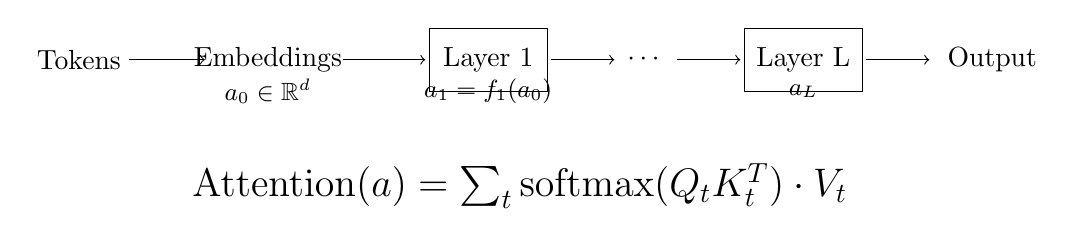
\begin{tikzpicture}[scale=0.8]
    % Tokens
    \node at (0,0) {Tokens};
    \draw[->] (0.8,0) -- (2,0);
    
    % Embeddings
    \node at (3,0) {Embeddings};
    \node at (3,-0.5) {\small $a_0 \in \mathbb{R}^d$};
    \draw[->] (4.2,0) -- (5.5,0);
    
    % Layers
    \node[draw,minimum width=1.5cm,minimum height=0.8cm] at (6.5,0) {Layer 1};
    \node at (6.5,-0.5) {\small $a_1 = f_1(a_0)$};
    \draw[->] (7.5,0) -- (8.5,0);
    
    \node at (9,0) {$\cdots$};
    \draw[->] (9.5,0) -- (10.5,0);
    
    \node[draw,minimum width=1.5cm,minimum height=0.8cm] at (11.5,0) {Layer L};
    \node at (11.5,-0.5) {\small $a_L$};
    \draw[->] (12.5,0) -- (13.5,0);
    
    \node at (14.5,0) {Output};
    
    % Attention equation
    \node at (7,-2) {\Large $\text{Attention}(a) = \sum_t \text{softmax}(Q_t K_t^T) \cdot V_t$};
\end{tikzpicture}
\end{center}

\vspace{0.5cm}
Key Points:
\begin{itemize}
    \item Residual stream: Information highway
    \item Each layer reads ALL previous tokens
    \item Autoregressive: One token at a time
\end{itemize}
\end{frame}

\begin{frame}
\frametitle{The Key Discovery}
\framesubtitle{Attention = Gradient Descent}

\begin{center}
\Large
\textbf{Click:} \href{run:./papers/2212.07677_transformers_gradient_descent.pdf}{\color{blue}von Oswald et al. 2022}
\end{center}

\vspace{0.5cm}

\begin{block}{Main Result}
\Large
\begin{equation*}
\text{Linear Self-Attention} = a + \eta \cdot \nabla \mathcal{L}
\end{equation*}
\end{block}

\vspace{0.5cm}
\textbf{Attention literally computes gradients!}

\begin{itemize}
    \item Single layer = one gradient step (exact!)
    \item Multi-layer = preconditioned gradient descent
    \item Not approximation -- mathematically exact
\end{itemize}
\end{frame}

% ==========================================
% SECTION 4: Interpretability (2.5 min)
% ==========================================

\begin{frame}
\frametitle{What We've Found Inside}
\framesubtitle{Mechanistic Interpretability}

\textbf{1. Induction Heads} (Anthropic)
\begin{itemize}
    \item Pattern completion circuits
    \item Emerge at $\sim$2.5B tokens
    \item \href{run:./papers/transformer_circuits_monosemantic_2023.md}{\color{blue}See visualization}
\end{itemize}

\vspace{0.3cm}
\textbf{2. Function Vectors} 
\begin{itemize}
    \item Tasks = directions in activation space
    \item \href{run:./papers/2310.15213_function_vectors.pdf}{\color{blue}Todd et al. 2024}
    \item Arithmetic: $v_{\text{translate}} + v_{\text{formal}} = v_{\text{formal translation}}$
\end{itemize}

\vspace{0.3cm}
\textbf{3. Superposition}
\begin{itemize}
    \item Many "programs" in same weights
    \item Examples select which program
    \item \href{run:./papers/transformer_circuits_scaling_2024.md}{\color{blue}Anthropic 2024}
\end{itemize}
\end{frame}

\begin{frame}
\frametitle{Layer-Wise Processing}
\framesubtitle{Information Flow Through Depth}

\begin{center}
\Large
\textbf{Click:} \href{run:./papers/2211.15661_learning_algorithm.pdf}{\color{blue}Akyürek et al. 2022}
\end{center}

\vspace{0.5cm}

\begin{center}
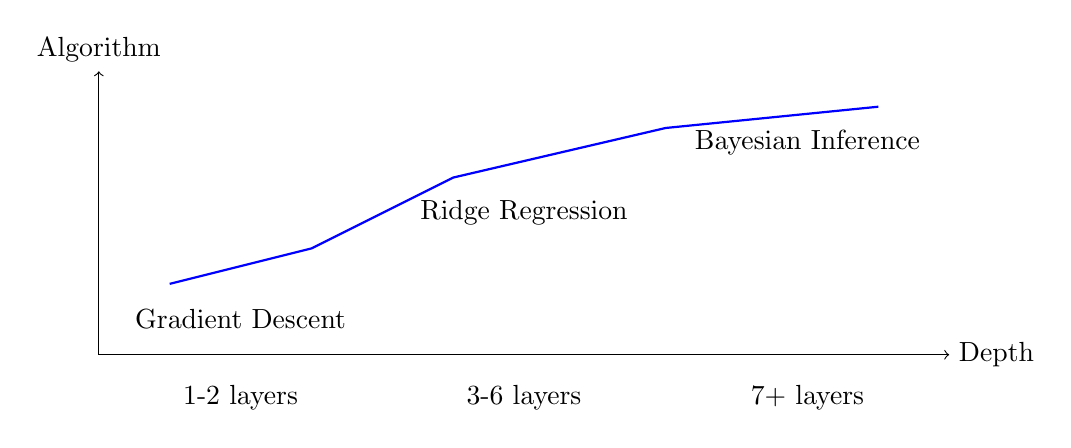
\begin{tikzpicture}[scale=0.9]
    \draw[->] (0,0) -- (12,0) node[right] {Depth};
    \draw[->] (0,0) -- (0,4) node[above] {Algorithm};
    
    \draw[thick,blue] (1,1) -- (3,1.5) -- (5,2.5) -- (8,3.2) -- (11,3.5);
    
    \node at (2,0.5) {Gradient Descent};
    \node at (6,2) {Ridge Regression};
    \node at (10,3) {Bayesian Inference};
    
    \node[below] at (2,-0.3) {1-2 layers};
    \node[below] at (6,-0.3) {3-6 layers};
    \node[below] at (10,-0.3) {7+ layers};
\end{tikzpicture}
\end{center}

\textbf{Phase transitions with depth!}
\end{frame}

% ==========================================
% SECTION 5: Mathematical Constructions (2 min)
% ==========================================

\begin{frame}
\frametitle{What Can Transformers Provably Do?}
\framesubtitle{Mathematical Limits}

\textbf{Proven Capabilities:}
\begin{enumerate}
    \item \textbf{Gradient Descent} -- Exact implementation
    \item \textbf{Ridge Regression} -- Medium depth
    \item \textbf{Bayesian Inference} -- Deep networks
    \item \textbf{Universal Computation} -- Turing complete!
\end{enumerate}

\vspace{0.5cm}
\textbf{Recent Result (2024):}
\begin{itemize}
    \item Prompting itself is Turing-complete
    \item \href{run:./papers/2411.01992_prompting_turing_complete.pdf}{\color{blue}Click for paper}
\end{itemize}

\vspace{0.5cm}
\textbf{Memory Bounds:}
\begin{itemize}
    \item $\Theta(n)$ capacity for $n$ examples
    \item \href{run:./papers/2405.13718_memory_capacity.pdf}{\color{blue}Tian et al. 2024}
\end{itemize}
\end{frame}

% ==========================================
% SECTION 6: Mesa-Optimization (2.5 min)
% ==========================================

\begin{frame}
\frametitle{Mesa-Optimization}
\framesubtitle{Two Optimization Loops}

\begin{center}
\Large
\textbf{Click:} \href{run:./papers/1906.01820_risks_learned_optimization.pdf}{\color{blue}Hubinger et al. 2019} | 
\href{run:./papers/2309.05858_mesa_optimization.pdf}{\color{blue}von Oswald et al. 2023}
\end{center}

\vspace{0.5cm}

\begin{center}
\begin{tabular}{|l|l|l|}
\hline
& \textbf{OUTER (Training)} & \textbf{INNER (Inference)} \\
\hline
Optimizer & SGD on parameters $\theta$ & Attention implements GD \\
\hline
Objective & Training loss & In-context loss \\
\hline
Updates & Weights & Activations \\
\hline
Time & Months & Single forward pass \\
\hline
\end{tabular}
\end{center}

\vspace{0.5cm}
\textbf{Critical insight:} Model learns HOW to learn, not just WHAT to predict

\vspace{0.3cm}
\textbf{Emerges without design!} Never explicitly trained for optimization
\end{frame}

\begin{frame}
\frametitle{Mesa-Optimization Evidence}
\framesubtitle{Internal Optimizer Discovery}

\begin{center}
\Large
\textbf{Click:} \href{run:./papers/2309.05858_mesa_optimization.pdf}{\color{blue}Uncovering Mesa-Optimization}
\end{center}

\vspace{0.5cm}

Two-stage process discovered:
\begin{enumerate}
    \item \textbf{Early layers:} Preconditioning
    \item \textbf{Later layers:} Optimization on preconditioned problem
\end{enumerate}

\vspace{0.5cm}
Key findings:
\begin{itemize}
    \item Autoregressive training $\rightarrow$ internal optimizers
    \item Generalizes to unseen tasks
    \item Can extract the learned algorithm
\end{itemize}
\end{frame}

% ==========================================
% SECTION 7: Grad Student Analogy (1.5 min)
% ==========================================

\begin{frame}
\frametitle{Why Few-Shot Works}
\framesubtitle{The Grad Student Analogy}

\Large
\textbf{Few-shot learning $\approx$ Supervising grad students}

\vspace{0.5cm}
\normalsize
\begin{enumerate}
    \item \textbf{Examples provide new information}
    \begin{itemize}
        \item Your specific notation
        \item Not in training data
    \end{itemize}
    
    \item \textbf{Computable format}
    \begin{itemize}
        \item Examples $>$ descriptions
        \item Model runs gradient descent on them
    \end{itemize}
    
    \item \textbf{Disambiguate task}
    \begin{itemize}
        \item "Prove like Bourbaki, not Arnold"
    \end{itemize}
    
    \item \textbf{Knowledge loading (push system)}
    \begin{itemize}
        \item Examples activate circuits
        \item Weights $\rightarrow$ activations
    \end{itemize}
\end{enumerate}

\vspace{0.5cm}
\textit{Examples are training data for the internal optimizer!}
\end{frame}

% ==========================================
% Conclusion (0.5 min)
% ==========================================

\begin{frame}
\frametitle{Conclusion}
\framesubtitle{The Key Insight}

\begin{center}
\Large
\textbf{Few-shot learning works because transformers are computers that run learning algorithms}
\end{center}

\vspace{1cm}

\begin{itemize}
    \item Your examples are the \textbf{program}
    \item The forward pass is the \textbf{execution}
    \item The output is the result of \textbf{internal optimization}
\end{itemize}

\vspace{1cm}

\begin{center}
\textbf{This isn't metaphorical -- it's mathematically proven}
\end{center}
\end{frame}

% ==========================================
% Q&A Slide
% ==========================================

\begin{frame}
\frametitle{Questions?}
\framesubtitle{15-minute Q\&A}

\Large
\textbf{Appendix Topics Available:}

\normalsize
\begin{itemize}
    \item A1: Detailed mechanistic interpretability
    \item A2: Statistical learning theory connection
    \item A3: Test-time training advances
    \item A4: Prompt engineering theory
    \item A5: Failure modes and limitations
\end{itemize}

\vspace{0.5cm}
\textbf{Key Papers:}
\begin{itemize}
    \item \href{run:./papers/2212.07677_transformers_gradient_descent.pdf}{\color{blue}von Oswald 2022} -- Gradient descent proof
    \item \href{run:./papers/2309.05858_mesa_optimization.pdf}{\color{blue}von Oswald 2023} -- Mesa-optimization
    \item \href{run:./papers/2211.15661_learning_algorithm.pdf}{\color{blue}Akyürek 2022} -- Algorithm identification
    \item \href{run:./papers/1906.01820_risks_learned_optimization.pdf}{\color{blue}Hubinger 2019} -- Original mesa concept
\end{itemize}
\end{frame}

% ==========================================
% APPENDIX SLIDES (for Q&A)
% ==========================================

\begin{frame}
\frametitle{A1: Mechanistic Interpretability Details}
\framesubtitle{Circuit Discovery}

\textbf{Induction Heads:}
\begin{itemize}
    \item Previous token head + induction head
    \item Implements $[A][B] \ldots [A] \rightarrow [B]$
    \item \href{run:./papers/transformer_circuits_monosemantic_2023.md}{\color{blue}Anthropic analysis}
\end{itemize}

\vspace{0.5cm}
\textbf{Sparse Autoencoders:}
\begin{itemize}
    \item Extract monosemantic features
    \item Reveals superposition
    \item \href{run:./papers/transformer_circuits_scaling_2024.md}{\color{blue}Scaling study}
\end{itemize}

\vspace{0.5cm}
\textbf{Knowledge Circuits:}
\begin{itemize}
    \item Early: Query formation
    \item Middle: Knowledge retrieval
    \item Late: Answer formatting
\end{itemize}
\end{frame}

\begin{frame}
\frametitle{A2: Statistical Learning Theory}
\framesubtitle{Generalization Guarantees}

\textbf{PAC Bounds via Stability:}
\begin{itemize}
    \item Excess risk: $|R(T) - \hat{R}(T)| \leq 2L\sqrt{\frac{\log(2/\delta)}{2M}}$
    \item \href{run:./papers/mlr_press_li2023.md}{\color{blue}Li et al. 2023}
\end{itemize}

\vspace{0.5cm}
\textbf{Rademacher Complexity:}
\begin{itemize}
    \item Sequence-length independent bounds
    \item Explains why models don't overfit to examples
    \item \href{run:./papers/games_automata_vc_dimension.md}{\color{blue}Classical theory connection}
\end{itemize}

\vspace{0.5cm}
\textbf{Minimax Optimality:}
\begin{itemize}
    \item Rate: $O(n^{-\beta/(2\beta+d)})$ for $\beta$-smooth functions
    \item \href{run:./papers/2408.12186_minimax_optimal.pdf}{\color{blue}2024 result}
\end{itemize}
\end{frame}

\begin{frame}
\frametitle{A3: Test-Time Training}
\framesubtitle{Explicit Optimization at Inference}

\begin{center}
\Large
\textbf{Click:} \href{run:./papers/2503.11842_test_time_training.pdf}{\color{blue}Test-Time Training (2025)}
\end{center}

\vspace{0.5cm}

\textbf{Idea:} Gradient updates on context examples during inference

\vspace{0.5cm}
\textbf{Benefits:}
\begin{itemize}
    \item Combines parametric + non-parametric learning
    \item Better sample complexity
    \item Provable improvements
\end{itemize}

\vspace{0.5cm}
\textbf{Connection:} Makes mesa-optimization explicit!
\end{frame}

\begin{frame}
\frametitle{A4: Prompt Engineering Theory}
\framesubtitle{Optimal Example Selection}

\textbf{Determinantal Point Processes:}
\begin{itemize}
    \item $P(S) \propto \det(K_S)$
    \item Balances similarity and diversity
    \item \href{run:./papers/acl_coverage_based_selection.md}{\color{blue}Coverage-based selection}
\end{itemize}

\vspace{0.5cm}
\textbf{Order Effects:}
\begin{itemize}
    \item Entropy ordering works best
    \item 17-point improvement on compositional tasks
    \item \href{run:./papers/2402.07927_prompt_engineering_survey.pdf}{\color{blue}Survey paper}
\end{itemize}

\vspace{0.5cm}
\textbf{OPRO (LLMs as Optimizers):}
\begin{itemize}
    \item Natural language optimization
    \item 50\% improvement on reasoning
    \item \href{run:./papers/2309.03409_llms_as_optimizers.pdf}{\color{blue}Yang et al. 2023}
\end{itemize}
\end{frame}

\begin{frame}
\frametitle{A5: Failure Modes}
\framesubtitle{When Few-Shot Doesn't Help}

\textbf{Limitations:}
\begin{enumerate}
    \item \textbf{Context window constraints}
    \begin{itemize}
        \item Memory: $\Theta(n)$ for $n$ examples
    \end{itemize}
    
    \item \textbf{Task misalignment}
    \begin{itemize}
        \item Mesa-objective $\neq$ your objective
    \end{itemize}
    
    \item \textbf{Distribution shift}
    \begin{itemize}
        \item Examples not representative
    \end{itemize}
    
    \item \textbf{Adversarial examples}
    \begin{itemize}
        \item Can hijack internal optimizer
    \end{itemize}
\end{enumerate}

\vspace{0.5cm}
\textbf{When it fails:}
\begin{itemize}
    \item Novel capabilities not in training
    \item Contradictory examples
    \item Tasks requiring true reasoning (not pattern matching)
\end{itemize}
\end{frame}

\begin{frame}
\frametitle{Additional Resources}
\framesubtitle{For Further Reading}

\textbf{Core Papers:}
\begin{itemize}
    \item \href{run:./papers/2005.14165_gpt3_language_models_few_shot.pdf}{\color{blue}GPT-3} -- Original few-shot benchmarks
    \item \href{run:./papers/2303.08774_gpt4_technical_report.pdf}{\color{blue}GPT-4} -- Modern performance
    \item \href{run:./papers/2309.16583_gpt_fathom.pdf}{\color{blue}GPT-Fathom} -- Model comparisons
\end{itemize}

\vspace{0.5cm}
\textbf{Theory Papers:}
\begin{itemize}
    \item \href{run:./papers/1912.10077_universal_approximators.pdf}{\color{blue}Universal approximation}
    \item \href{run:./papers/1901.03429_turing_completeness.pdf}{\color{blue}Turing completeness}
    \item \href{run:./papers/2306.04637_transformers_statisticians.pdf}{\color{blue}Transformers as statisticians}
\end{itemize}

\vspace{0.5cm}
\textbf{Practical Guides:}
\begin{itemize}
    \item \href{run:./papers/prompthub_few_shot_guide.md}{\color{blue}Few-shot prompting guide}
    \item \href{run:./papers/analytics_vidhya_comparison.md}{\color{blue}Zero vs few-shot comparison}
\end{itemize}
\end{frame}

\end{document}